\documentclass[main]{subfiles}
\begin{document}

\section{Introduction}
%@@@@@@@@@@@@@@@@@@@@@@@@@@@@@@
% summarizes lecture 1
% author: Benjamin Ellenberger & Joachim Ott

\subsection{Semiconductors}
In case you have trouble understanding the concepts of device physics, then please refer to the appended slide set on device physics in chapter \ref{sec:dev-physics}.

%Ben Start
Semiconductors and other materials are arranged in regular structures, so called crystals. The outermost electrons of the atoms, the valence electrons, are distributed in a way that defines and holds together the structure of the crystal.

\begin{figure}[H]
\centering
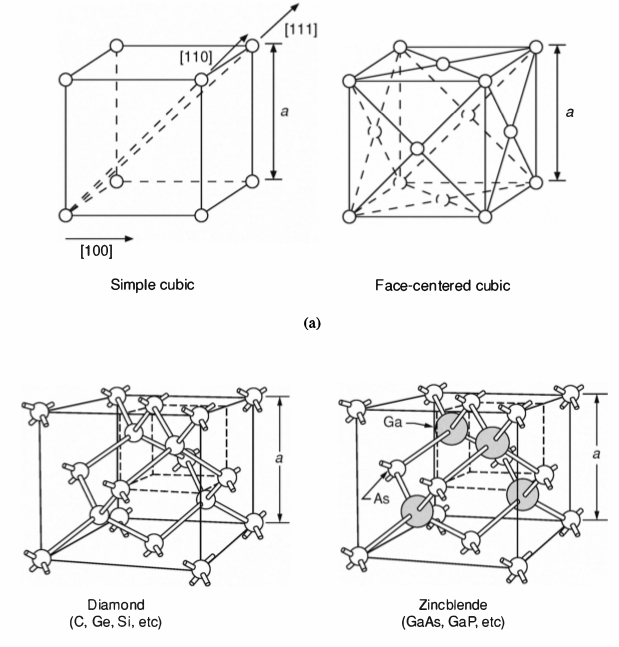
\includegraphics[scale=0.3]{pics/crystal_structure.png}
\caption{Crystal structure of important semiconductors. a) Possibilities of arrangement. b) Arrangement of silicon (Si) and Gallium arsenide (GaAs). Pure silicon crystallizes in a diamond crystal, Gallium arsenide crystallizes in a so called Zincblende structure \cite{book:VLSI}.}
\end{figure}

\subsection{Energy Band Diagrams}
We classify crystals and other solids according to their electrical conductivity into \textbf{insulators}, \textbf{semiconductors}, and \textbf{conductors or metals} in the order of increasing conductivity. Semiconductors are at an intermediate conductivity level, a special property making them suitable for transistors because their conductivity is tunable. It can be modulated by varying the electrical boundary conditions and by introducing atoms of foreign elements into the crystal structure (so called \textbf{impurity doping}).\\
The conductivity of a solid is dependent on the amount of mobile electrons in the solid. Electrons can either be bound to an ion or can be mobile within the solid. Electrical currents are then carried by the motion of the mobile valence electrons. In order to be mobile, the electrons must acquire a minimum energy to break free. The electrons in solids can only be in certain ranges, so called \textbf{energy bands}, and must avoid the forbidden ranges, so called \textbf{energy gaps or band gaps}.

\begin{figure}[H]
\centering
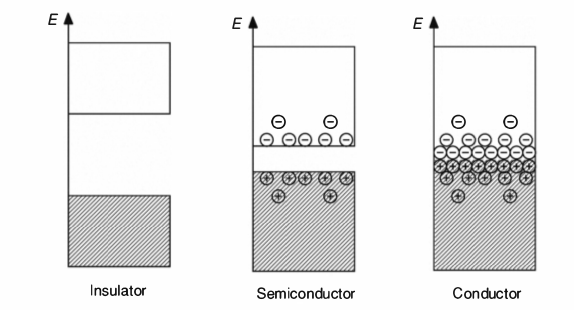
\includegraphics[scale=0.5]{pics/energybands.png}
\caption{The schematic energy bands of an insulator, a semiconductor and a conductor. The hatched areas symbolize the states that are occupied by electrons at zero temperature. At non-zero temperature, some electrons occupy higher energy states leaving ''holes'' in the unoccupied lower-energy states. For insulators, the energy bands are either completely filled or empty, as all electrons are bound. A semiconductor has almost full or almost empty bands and the current can only flow under certain conditions. A conductor has partly filled bands within which electrons can move. }
\end{figure}

Valence bands in semiconductors are almost filled, conductance bands almost empty. A concept simplifying the view on semiconductors is that unoccupied states in a valence band are denoted a holes, being positively charged particles.

\begin{figure}[H]
\centering
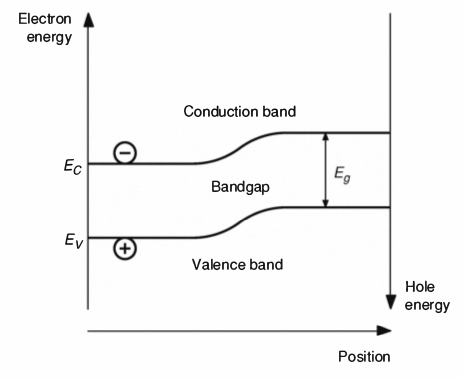
\includegraphics[scale=0.5]{pics/bandgap.png}
\caption{Valence and conduction band of a semiconductor. The energy is plotted as a function of position in one dimension. The energy of the band gap \(E_g\) denotes the difference between the lowest conduction band energy and the highest valence band energy. The band edges tell us the minimum amount of energy an electron has to acquire or lose to bridge the bandgap.}
\end{figure}

\subsection{Carrier concentrations at Thermal equilibrium}
Thermal energy makes some electrons move from the lower-energy states to the higher-energy states. The occupancy of energy states is described by the \textbf{Fermi-Dirac distribution} (\(E_F\) denotes the \textbf{Fermi level}, the energy at which the occupation probability is 0.5, k= Boltzmann constant, T=absolute Temperature).

\begin{align*}
F(E) = \frac{1}{1+e^{\frac{E-E_F}{kT}}}
\end{align*}

Typical impurity doping concentration, \(E_F\) is well separated from the valence and conduction band edges (\(|E-E_F| >> kT\)), thus we can use the Boltzmann distribution
\begin{align*}
F(E) = e^{-\frac{E-E_F}{kT}}
\end{align*}
This probability distribution is the reason for the exponential characteristics of diodes and transistors. The fermi level in an undoped semiconductor is usually halfway between the valence and conduction band.

\subsection{Impurity doping}

The conductivity of a semiconductor is increased significantly by impurity doping. By replacing several atoms of the semiconductor crystal structure by a different element (a donor impurity if it has a valence electron more, an acceptor impurity if it has a valence electron less than the semiconductor atom), we get more unbound electrons/holes as the impurity atom itself is electrically neutral and the electron/hole can move freely.

\begin{figure}[H]
\centering
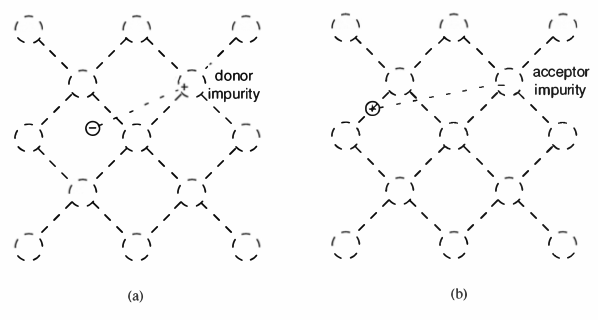
\includegraphics[scale=0.4]{pics/impurity_doping.png}
\caption{Semiconductor with a) donor and b) acceptor impurity doping. The excess charge carrier is only loosely bound to the ion cores (dashed circles).}
\end{figure}

The introduction of donors moves the Fermi level from near the center of the bandgap further towards the conduction-band edge, whereas the
introduction of acceptors moves it closer to the valence-band edge. Higher acceptor doping semiconductors are called \textbf{n-type}, higher donor doping semiconductors are called \textbf{p-type}. Too strongly doped semiconductors have a Fermi level within the valence or conductance band and therefore are similar to metals. Common doping elements are phosphorus (P), arsenic (As) as donors and boron (B) as acceptor.\\
The mobile charge carriers that are dominant in the semiconductor in thermal equilibrium are the majority carriers, the sparser ones are the minority carriers.

\subsection{Current densities}
By historical definition the electron is assigned the negative elementary charge \(-q\) , where we define \(q\) to be positive. However, the direction of the current density is
defined as the direction of positive charge flow. For each carrier type the current flow is due to two basic mechanisms, namely diffusion and drift.\\
Diffusion is a term borrowed from gas dynamics. It describes the process by which a net particle flow is directed from a region of
higher particle density to a region of lower particle density along the density gradient. As we shall see, diffusion determines the current flow in diodes and, within the operating range mainly considered here, in transistors.
Diffusion also governs the ion flows in biological neurons.\\
Drift currents are caused by electric fields.

\subsection{p-n Junction Diode}
The fundamental semiconductor device is the p-n junction diode. It is built from an n-type semiconductor and a p-type semiconductor, which, when brought into physical contact, give rise to a net electron flow from n-type to p-type region and a net hole flow from p-type to n-type region. The diffusing minority carriers recombine with majority carriers in the vicinity of the junction and therefore gets depleted of mobile charge carriers, hence its name \textbf{depletion region or space-charge region}. 

\begin{figure}[H]
\centering
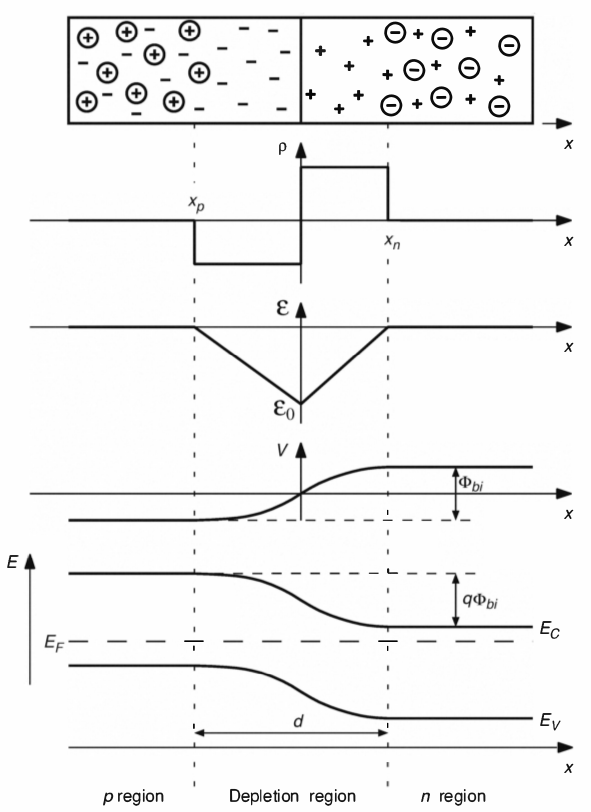
\includegraphics[scale=0.4]{pics/depletion_region.png}
\caption{Characteristics of an abrupt p-n junction in thermal equilibrium with space-charge distribution \(\rho\), electric field distribution \(\mathcal{E}\), potential distribution \(V\). and energy-band diagram \(E\).}
\end{figure}

The depletion region on the n-type side of the junction is depleted of donor electrons and has surplus protons, the p-type side of the junction is depleted of acceptor holes (filled with the donor electrons) and so have surplus electrons. This builds up an electric field pulling the majority carriers back into the other direction. In thermal equilibrium, diffusion and drift currents balance each other out and no net current flow is observed. The offset between the energy bands bordering the depletion region is an electrical potential called \textbf{built-in potential or diffusion potential \(\Phi_{bi}\)}.

\subsection{Forward and Reverse Bias}

In a p-n junction, a net current flow through the diode is generated by applying a potential difference to it. A positive voltage difference applied to the p-type region relative to the n-type region is called a \textbf{forward bias} and the corresponding current is called \textbf{forward current}, a positive voltage difference applied to the n-type region relative to the p-type is called a \textbf{reverse bias}, and the corresponding current \textbf{reverse current}. In a steady state, the total current density must be constant throughout the diode. The electron current in the n-type region is transformed into a hole current in the p-type region. The applied voltage \(V\) appears across the depletion region as a change in the built-in voltage and thus modifies the width of the depletion region.\\
A \textbf{forward bias} shrinks the step across the junction. The positive potential applied to the p-type material repels the holes, while the negative potential applied to the n-type material repels the electrons. With increasing forward-bias voltage, the depletion zone eventually becomes thin enough that the zone's electric field cannot counteract charge carrier motion across the p–n junction, as a consequence reducing electrical resistance. The electrons that cross the p–n junction into the p-type material (or holes that cross into the n-type material) will diffuse in the near-neutral region. The forward current in the p-n junction when it is forward-biased involves electrons from the n-type material moving across the junction and combining with holes in the p-type material. Electrons can then proceed further onward by jumping from hole to hole, so the holes can be said to be moving to the opposite direction in this process.

\begin{figure}[H]
\centering
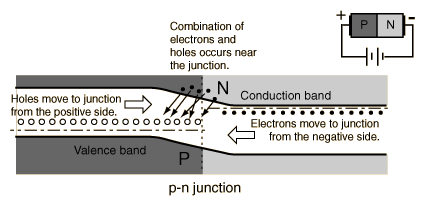
\includegraphics[scale=0.8]{pics/forward_bias.png}
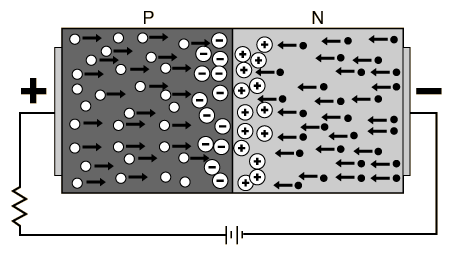
\includegraphics[scale=0.8]{pics/forward_bias2.png}
\caption{Forward biasing of an p-n junction.}
\end{figure}

A \textbf{reverse bias} expands the step across the junction. To reverse-bias the p-n junction, the p side is made more negative, making it "uphill" for electrons moving across the junction. This will cause a transient current to flow as both electrons and holes are pulled away from the junction. When the potential formed by the widened depletion layer equals the applied voltage, the current will cease except for the small thermal current.

\begin{figure}[H]
\centering
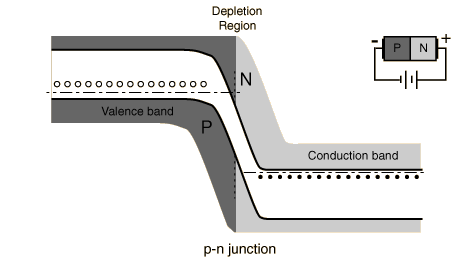
\includegraphics[scale=0.8]{pics/reverse_bias.png}
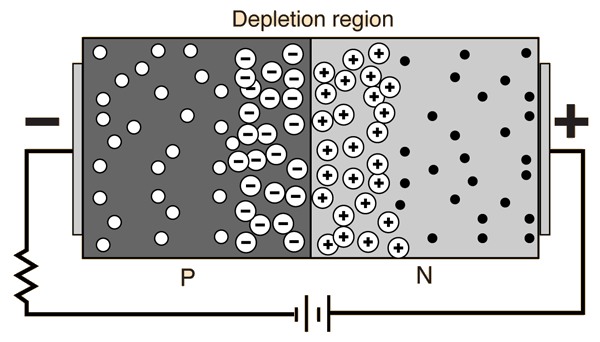
\includegraphics[scale=0.6]{pics/reverse_bias2.png}
\caption{Reverse biasing of an p-n junction.}
\end{figure}

\begin{figure}[H]
\centering
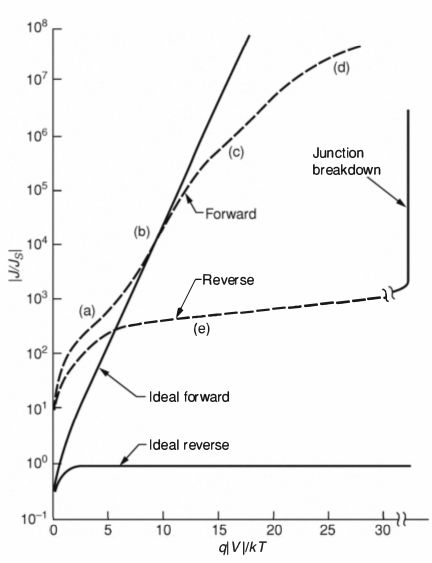
\includegraphics[scale=0.5]{pics/biasing.png}
\caption{Biasing of an p-n junction.}
\end{figure}

For large reverse biases, a phenomenon called \textbf{junction breakdown} occurs that expresses itself in a sudden increase of reverse current at a certain reverse voltage. For silicon with typical impurity doping concentrations this effect is due to impact ionization: The generation of electron-hole pairs by collision with an electron or hole that has acquired sufficient kinetic energy in the electric field of the depletion region. A charge carrier may create multiple electron-hole pairs during its transition through the depletion region. The generated carriers can in turn create electron-hole pairs if they acquire sufficient energy, and
so on. This effect is known as avalanche multiplication.

%Ben End

%Joachim Start
\subsection{MOS Transistor Structure}
\subsubsection{MIS}  Metal-Insulator-Semiconductor, consists of a conductor and a semiconductor, separated by thin insulation layer.
\subsubsection{MOS}  Metal-Oxide-Silicon, a version of MIS, in which silicon dioxide ($SiO_2$) is used as oxide.
\subsubsection{CMOS}  Complementary Metal Oxide Silicon, a MOS process in which both nFET and pFET are fabricated on the same substrate.
\subsubsection{MOSFET} Metal-Oxide-Semiconductor Field-Effect Transistor, built using MOS and a p-n junction diode.

\begin{figure}[htbp]
  \centering
  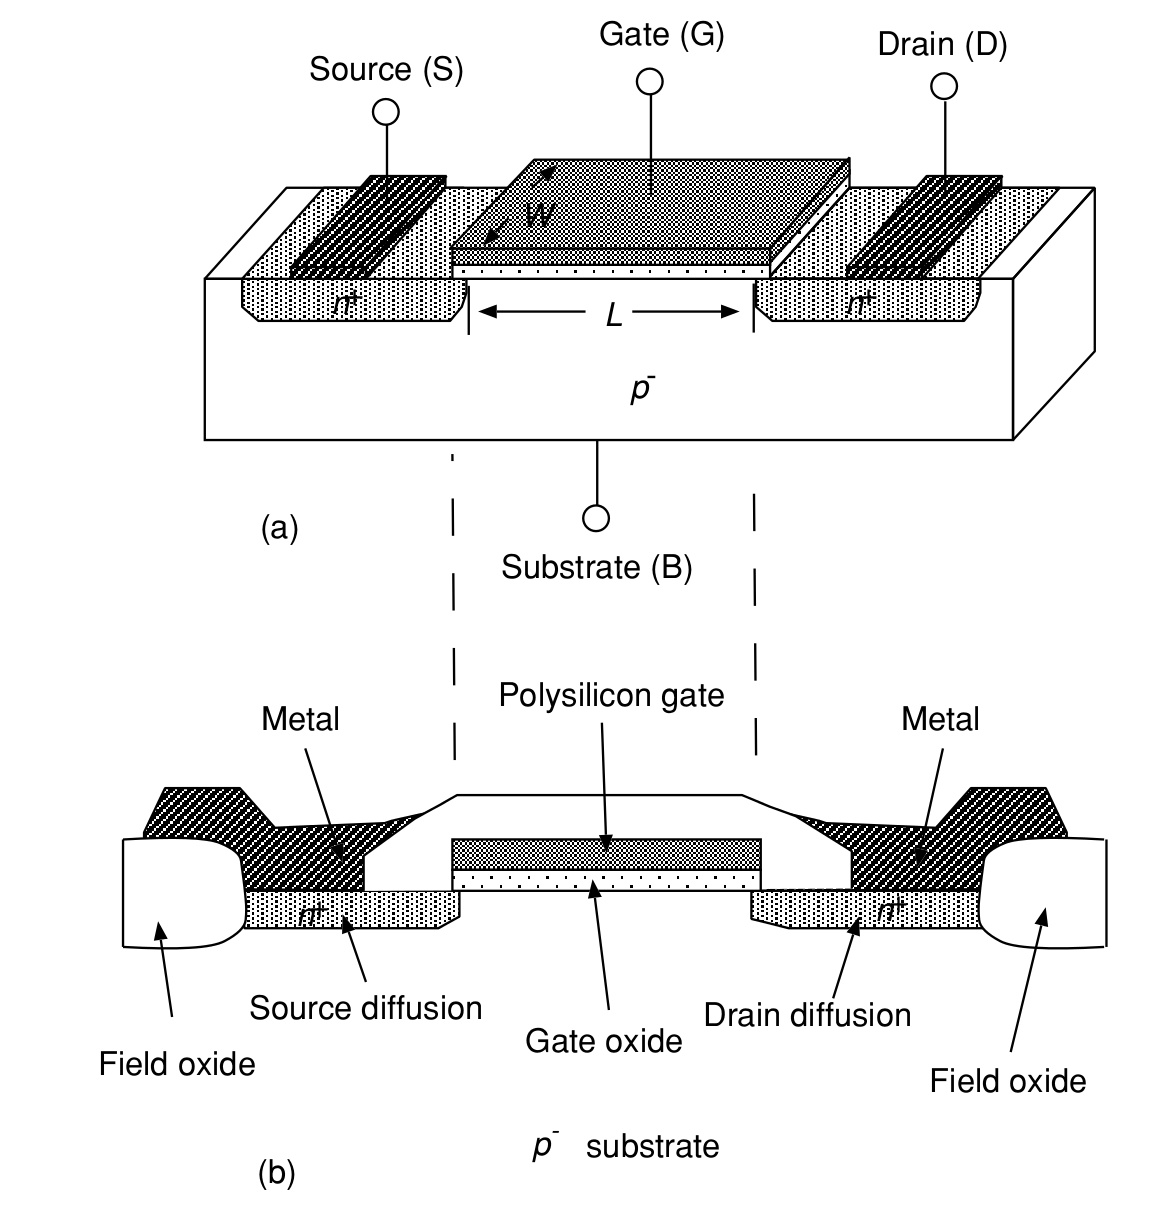
\includegraphics[scale=0.8]{pics/MOSFET_Structure.jpg}
  \caption{Structure of an n-type MOSFET in a pbody. The MOSFET has four terminals; the drain (D), the source (S), the gate (G), and the bulk (B). (a) Pictorial view of the MOSFET. (b) A more realistic picture of a cross-section of a fabricated MOSFET. Note that the gate oxide is much thinner than the field oxide. \cite{book:VLSI}}
  \label{fig:MOSFET_Structure}
\end{figure}\bigskip

\bigskip\subsection{MOS Transistor Terminals}
We can view the transistor as having four terminals:
\begin{enumerate}
\item Gate (G)
\item Source (S)
\item Drain (D)
\item Bulk (B)
\end{enumerate}

\bigskip\subsection{MOS Transistor Types}
\subsubsection{n-type}
    Because the n+ source and drain regions can supply a lot of electrons to the channel, this device is called an n-channel MOSFET (nFET,n-type MOSFET, NMOS) \cite{book:VLSI}
\subsubsection{p-type}
   In p-channel MOSFET (pFET,p-type MOSFET, PMOS) , the charge in the channel is carried by holes supplied from the source and drain regions.
    
\bigskip\subsection{MOS Transistor in Substrate}
Most CMOS processes use a p-type starting substrate.  The nFETs rest in the common $p^-$ substrate, and the pFETs rest in
n-wells within the substrate as shown in Fig. \ref{fig:MOSFET_Physical_Structure}

\begin{figure}[htbp]
  \centering
  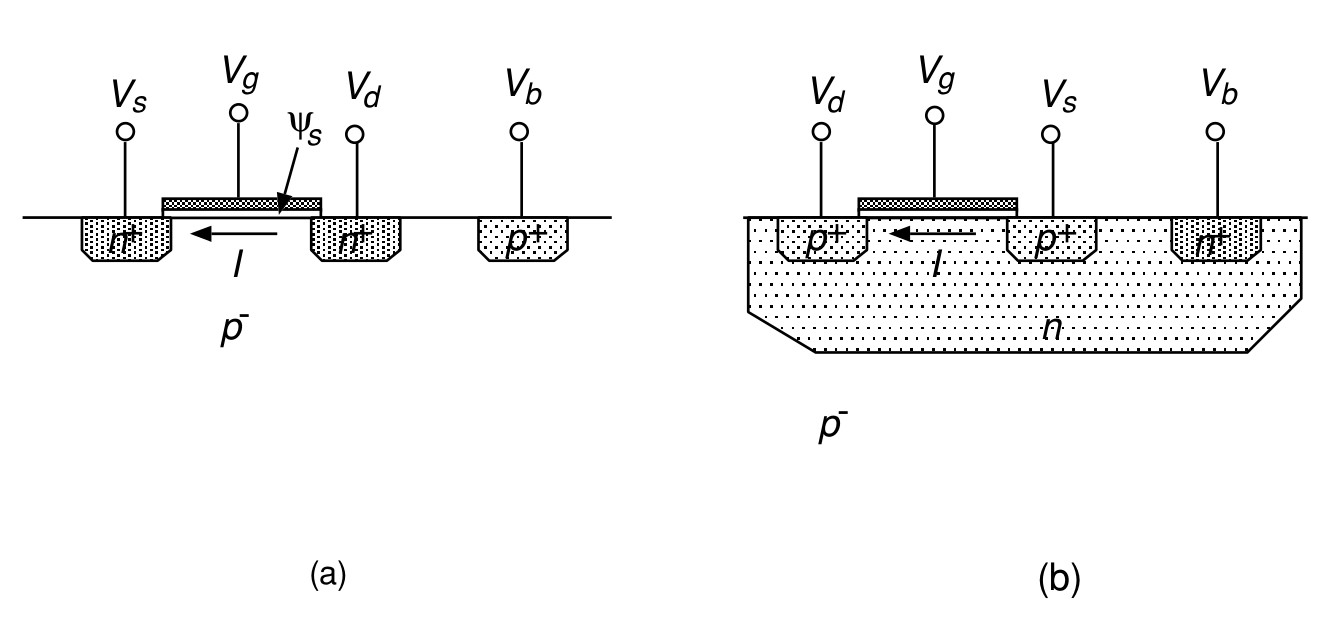
\includegraphics[scale=0.8]{pics/MOSFET_Physical_structure.jpg}
  \caption{Physical structure of (a) an nFET and (b) a pFET in a common $p^-$ substrate. The pFET rests in a n-well within the substrate. \cite{book:VLSI}}
  \label{fig:MOSFET_Physical_Structure}
\end{figure}

\bigskip\subsection{MOS Transistor Biasing}
\subsubsection{nFET}
To ensure only a small leakage current between the $n^+$ regions to the p-substrate, the junctions have to be reverse biased.
To do this, the drain voltage $V_d$ and the source voltage $V_s$ of the nFET should be greater than or equal to the bulk voltage $V_b$:
\begin{equation}
V_{sb}=V_s-V_b \geq 0
\end{equation}
\begin{equation}
V_{db}=V_d-V_b \geq 0
\end{equation}

The location of drain and source is defined by the carrier flow:\cite{book:VLSI}
\begin{itemize}
\item Electrons are supplied to the channel by the source, and removed by the drain.
\item Holes are supplied to the channel by the source, and removed by the drain.
\end{itemize}

The $n^+$ region biased at the higher voltage is called the drain, and the other $n^+$ region is called the source. Because electrons are negatively charged, the direction of positive current flow,
I, is from drain to source, even though the carriers flow from source to drain. \cite{book:VLSI}

\subsubsection{pFET}
In pFET , the $p^+$ regions should be biased negative relative to the bulk to reverse-bias the pn junctions.
\begin{equation}
V_{sb} \leq 0
\end{equation}
\begin{equation}
V_{db} \leq 0
\end{equation}

\subsection{MOS Transistor Channel}
The region underneath the gate and between the source and drain regions is called the channel. The channel has a width W, and a length L
. The channel is insulated from the gate above by a layer of silicon dioxide. The gate is made of heavily doped (low resistivity) polycrystalline silicon.
\cite{book:VLSI}

\subsection{MIS Operation Domains}
Depending on the charge of the gate, we either attract or repel majority carriers on the surface of the channel semiconductor.\\
\textbf{Important: }Relevant here is the type of substrate (p or n) the channel is made of, don't confuse it with nFET or pFET!
\begin{figure}[H]
  \centering
  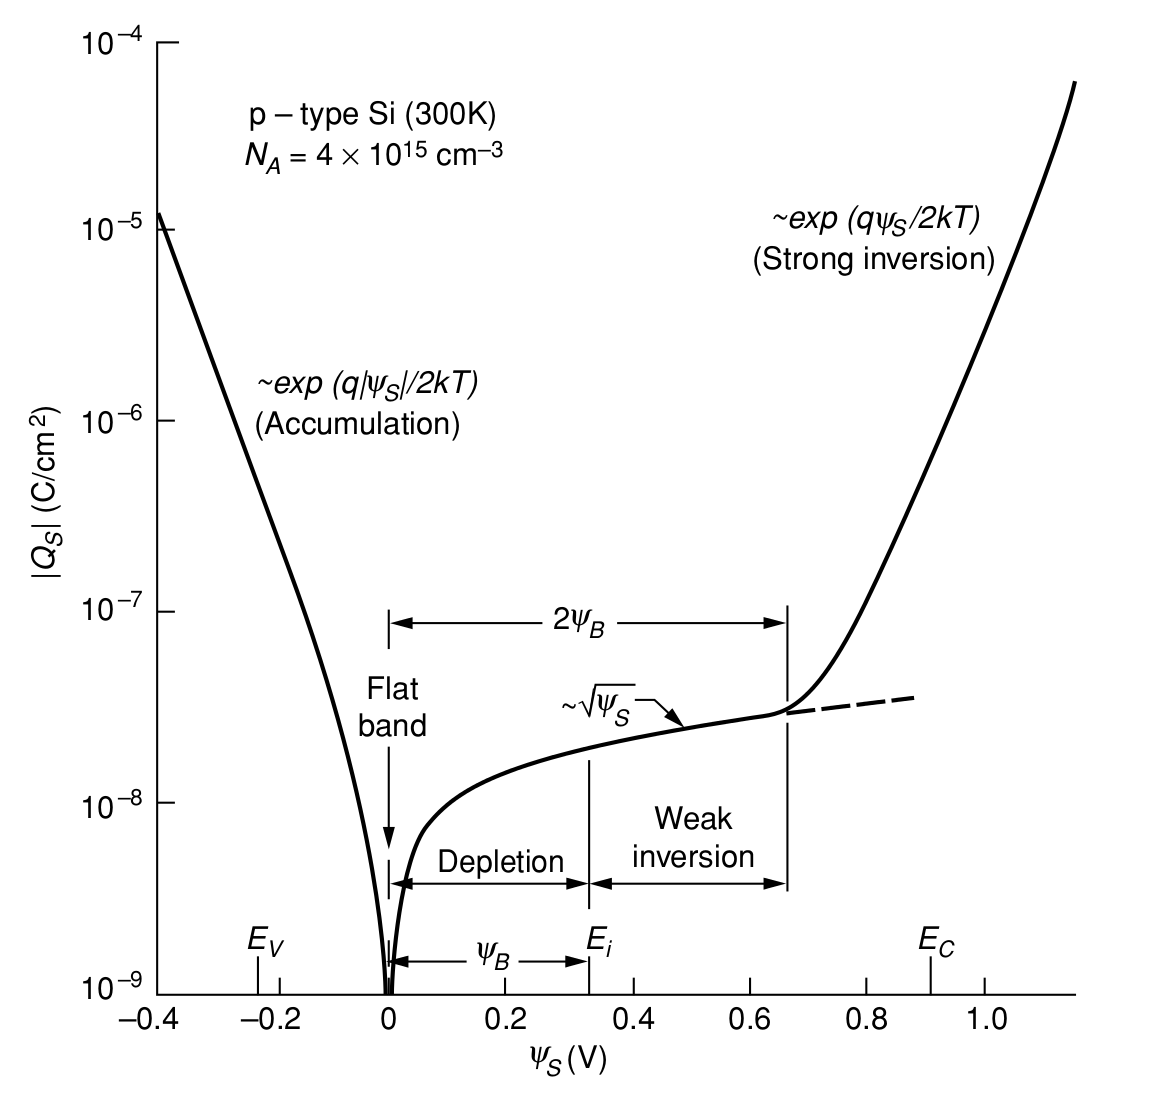
\includegraphics[scale=1]{pics/operation_domains.png}
  \caption{Dependence of the area charge $Q_s$ on the surface potential for p-type silicon with acceptor density $N_A = 4 \times 10^15cm^-3$ at room temperature. Figure adapted from S. M. Sze (1981), Physics of
Semiconductor Devices, 2nd Edition. \copyright 1981 by John Wiley $\&$ Sons, Inc.  \cite{book:VLSI}}
  \label{fig:coperation_domains}
\end{figure}

\subsubsection{Accumulated Transistor Channel}
Accumulation happens when a charge on the gate attracts a lot of majority carriers on the surface of the semiconductor underneath it.\\
For a p-substrate channel (default), as shown in figure \ref{fig:channel_accumulated}, a negative voltage on the gate means mobile electrons on the gate. These electrons (negatively charged) attract positive charges on the semiconductor surface underneath it, leading to accumulation of them. Since positive charges (holes) are the majority carrier in p-substrate, we call this situation accumulation.\\\\
In a n-substrate channel, positive charge on the gate leads to accumulation of electrons (majority carriers in n-substrate) on the channel surface.
\begin{figure}[H]
  \centering
  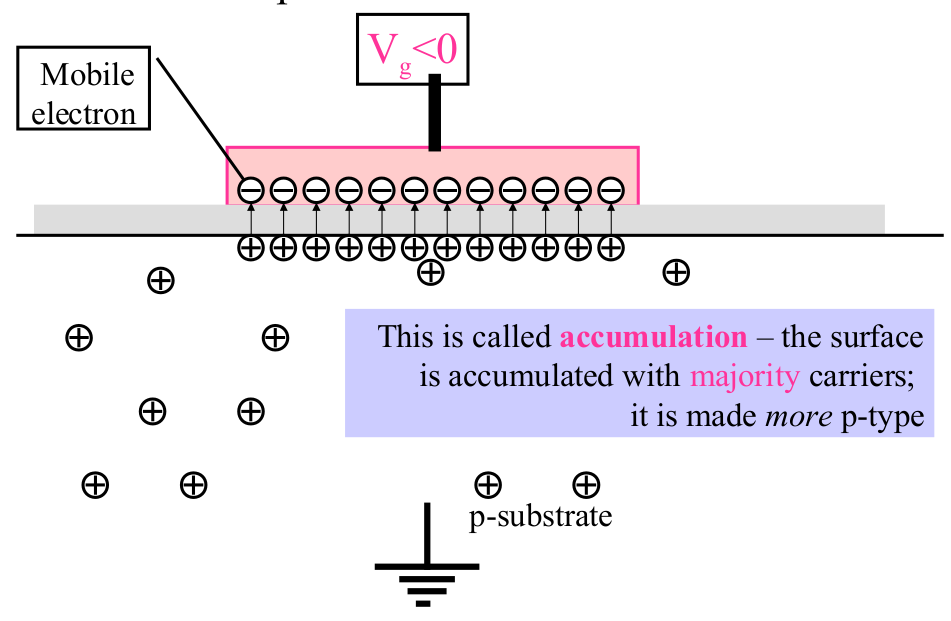
\includegraphics[scale=1]{pics/channel_accumulation.png}
  \caption{Accumulated Transistor Channel \cite{lec2}}
  \label{fig:channel_accumulated}
\end{figure}


\subsubsection{Flat-Band Transistor Channel}
In an ideal MIS diode, with no bias applied, the work function of the metal and the semiconductor are the same.  The Fermi levels line up and the energy bands in the semiconductor are flat. $\rightarrow$ Flat-Band Condition \cite{book:VLSI}\\
With $V_g=V_{fb}=0$, the majority carrier density is constant and equal to the dopant density.
\begin{figure}[H]
  \centering
  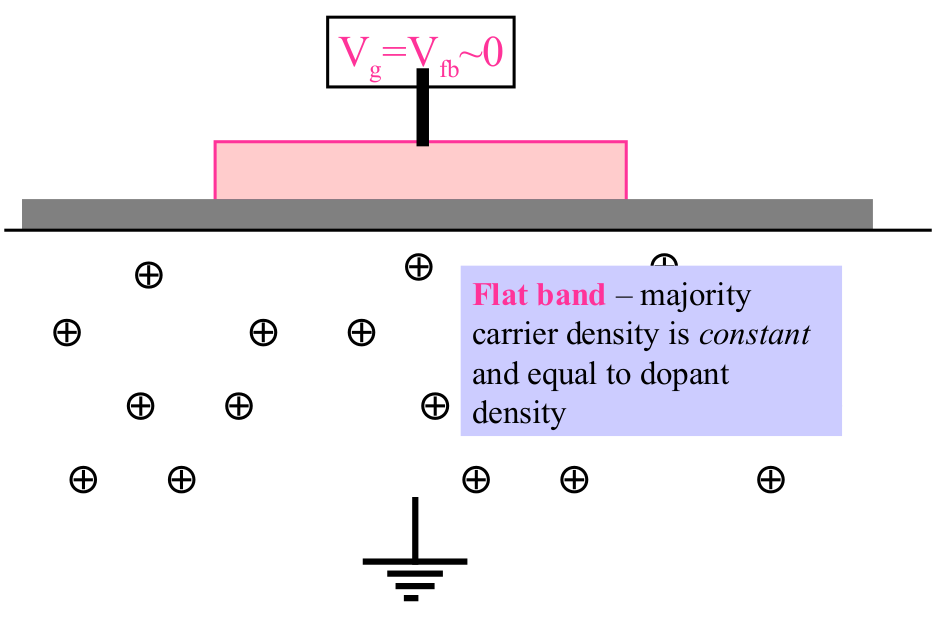
\includegraphics[scale=1]{pics/channel_flat_band.png}
  \caption{Flat-Band Transistor Channel \cite{lec2}}
  \label{fig:channel_flat_band}
\end{figure}

\subsubsection{Depleted Transistor Channel}

For a p-substrate channel, if we put a positive subthreshold voltage on the gate (positive charges), we repulse positive majority carriers on the semiconductor surface. $\rightarrow$ Depletion of majority carriers.\\
For a n-substrate channel, the same happens if we put a subthreshold negative charge on the gate. $\rightarrow$ Depletion of electrons (majority carrier in n substrate) on the semiconductor surface.

\begin{figure}[H]
  \centering
  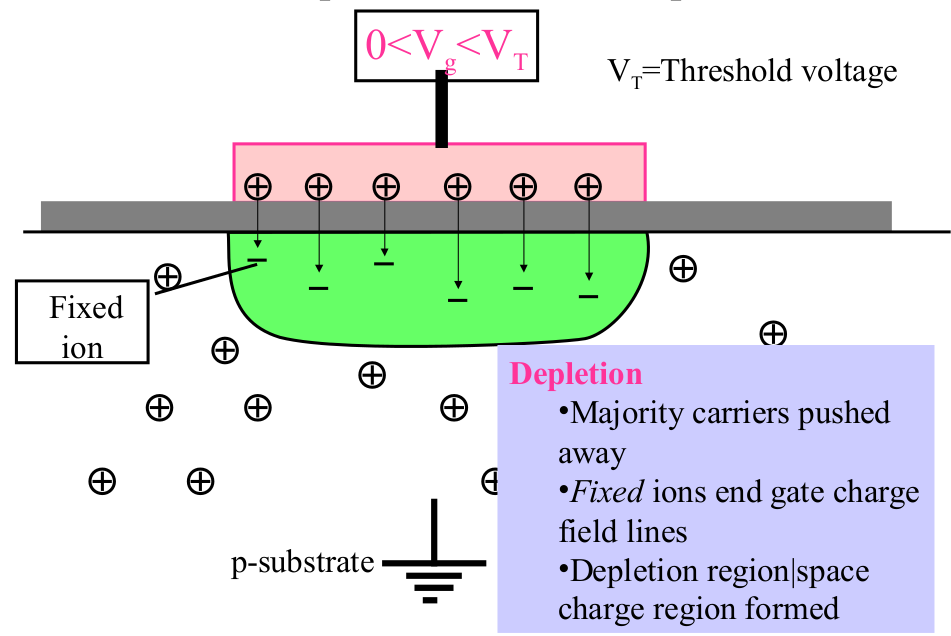
\includegraphics[scale=1]{pics/channel_depletion.png}
  \caption{Depleted Transistor Channel \cite{lec2}}
  \label{fig:channel_depletion}
\end{figure}

\subsubsection{Inverted Transistor Channel}
For a depleted p-substrate channel, if we now further increse the postive charge on the gate, we will reach a point where we start attracting negative minority carriers on the semiconductor surface. The surface becomes inverted. (p-type $\rightarrow$ n-type and vice versa in n substrate)  $\rightarrow$ Inversion
\begin{figure}[H]
  \centering
  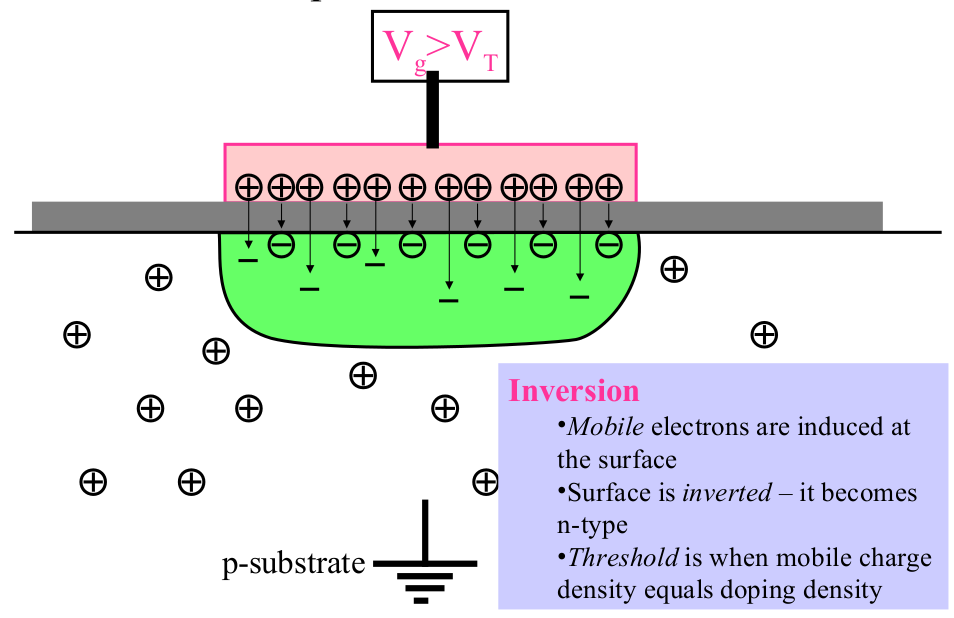
\includegraphics[scale=1]{pics/channel_inversion.png}
  \caption{Inverted Transistor Channel \cite{lec2}}
  \label{fig:channel_inversion}
\end{figure}

%Joachim End

\todo[inline]{Add more basic theory (e.g. definition and meaning of $U_T$)}
\end{document}